
\section{Architecture Integration}

\subsection{Model Support}

\begin{table}[H]
\centering
\small
\begin{tabular}{lllll}
\toprule
\textbf{Architecture} & \textbf{Attention class} & \textbf{Heads (H)} & \textbf{KV heads} & \textbf{Config} \\
\midrule
DistilBERT & \texttt{MultiHeadSelfAttention} & 12 & 12 (MHA) & Flat \\
RoBERTa & \texttt{BertSelfAttention} & 12 & 12 (MHA) & Nested \\
GPT-2 & \texttt{GPT2Attention} & 12 & 12 (MHA) & Causal \\
Qwen3.5 & \texttt{Qwen3Attention} & 8 & 2 (GQA) & GQA + RoPE \\
\bottomrule
\end{tabular}
\end{table}

GQA targets all four. For DistilBERT/RoBERTa/GPT-2 (all MHA), we reduce 
$H_{KV}$ from 12 to 6 by default. For Qwen3.5 (already GQA), we either 
preserve or further reduce.

\subsection{Weight Extraction}

\subsubsection{DistilBERT (Flat)}

DistilBERT has four projections:

\begin{lstlisting}
q_lin: Linear(768, 768)   # H = 12, d_h = 64
k_lin: Linear(768, 768)
v_lin: Linear(768, 768)
out_lin: Linear(768, 768)
\end{lstlisting}

\textbf{Extraction:} Direct. \texttt{q\_lin.weight} copied to \texttt{query.weight}, etc.

\textbf{Nested?} No. \texttt{out\_lin} is inside attention, so \texttt{is\_nested\_encoder = False}.

\subsubsection{RoBERTa (Nested)}

\begin{lstlisting}
attention.self.query: Linear(768, 768)
attention.self.key: Linear(768, 768)
attention.self.value: Linear(768, 768)
attention.output.dense: Linear(768, 768)
\end{lstlisting}

\textbf{Extraction:} From inner \texttt{self}. \texttt{attention.output.dense} is outside, so 
\texttt{is\_nested\_encoder = True} and we skip our own \texttt{out\_proj}.

\subsubsection{GPT-2 (Causal)}

\begin{lstlisting}
attn.c_attn: Conv1D(768, 2304)   # fused Q, K, V
attn.c_proj: Conv1D(768, 768)
\end{lstlisting}

\textbf{Extraction:} Transpose (Conv1D stores \texttt{(in, out)}) and split:

\begin{lstlisting}
w = src.c_attn.weight.t()  # (2304, 768)
q_w, k_w, v_w = w.chunk(3, dim=0)
\end{lstlisting}

\subsubsection{Qwen3.5 (GQA-native)}

\begin{lstlisting}
q_proj: Linear(1024, 2048)   # 8 heads $$\times$ 256
k_proj: Linear(1024, 512)    # 2 heads $$\times$ 256
v_proj: Linear(1024, 512)
o_proj: Linear(2048, 1024)
\end{lstlisting}

\textbf{Extraction:} Direct. Source is already GQA. If reducing $G$ from 2 to 1, 
we average the two KV heads.

\subsection{Injection Algorithm}

\textbf{Algorithm 3:} Inject GQA into a full model
\begin{lstlisting}
Input:  model M, config c, G (target KV heads)
Output: M with GQA-injected attention

1:  for   in transformer_layers(M) do
2:      src $\leftarrow$ extract_attention( )
3:      if src is None: continue
4:      H $\leftarrow$ num_query_heads(src)
5:      G $\leftarrow$ min(G, H)    Cannot exceed H
6:      G $\leftarrow$ largest_divisor(H, G)    Must divide H
7:      new $\leftarrow$ GQA(config=c, H=H, G=G)
8:      new.copy_weights(src)    See Algorithm 1
9:      replace_attention( , new)
10: end for
\end{lstlisting}

\subsection{Handling Special Cases}

\subsubsection{Grouping Factor}

For $H = 12$ and target $G = 5$, the algorithm snaps to $G = 4$ (largest 
divisor $\le$ 5). For $H = 12$ and $G = 7$, snaps to $G = 6$.

\subsubsection{Qwen3.5 with Existing GQA}

If the source is already GQA with $G_\text{src}$ heads and $G_\text{tgt} < G_\text{src}$, 
we regroup. If $G_\text{tgt} \ge G_\text{src}$, we keep the source configuration.

\subsubsection{Nested Encoder}

For RoBERTa, the outer \texttt{attention.output.dense} is preserved. Our GQA module 
returns context without applying \texttt{out\_proj}. The outer projection handles it.

\subsubsection{Causality}

For GPT-2 and Qwen, causal masking is applied:

\begin{lstlisting}
causal_tril = torch.tril(torch.ones((N_q, N_k)))
scores = scores.masked_fill(~causal_tril, -10000.0)
\end{lstlisting}

RoPE is applied to $Q, K$ before KV repetition, preserving causality.

\subsection{Safe Injection}

The \texttt{inject\_gqa} function returns \texttt{None} on failure:

\begin{lstlisting}
try:
    new_layer = GroupedQueryAttention(config=cfg, old_attn=curr_attn, ...)
except Exception as ex:
    logger.warning("Failed to instantiate GQA: %s", ex)
    return None
\end{lstlisting}

This allows the caller to skip the layer and continue with subsequent layers.

\subsection{Weight Transfer Correctness}

After \texttt{copy\_weights}, the following invariants hold:

\begin{enumerate}
\item \textbf{Query weights:} $W_Q^{(\text{new})} = W_Q^{(\text{old})}$ (exact).
\item \textbf{Output weights:} $W_O^{(\text{new})} = W_O^{(\text{old})}$ (exact).
\item \textbf{KV weights (MHA $\to$ GQA):} $W_K^{(\text{new})}_g = \frac{1}{r} \sum_{h \in g} W_K^{(\text{old})}_h$.
\item \textbf{Bias:} Copied where shapes match, zeroed otherwise.

\end{enumerate}
The \textbf{Frobenius norm} of each copied weight is checked to be $> 10^{-4}$, 
flagging silently broken copies.

\subsection{Parameter Count}

\begin{table}[H]
\centering
\small
\begin{tabular}{ll}
\toprule
\textbf{Configuration} & \textbf{Params ($W_Q + W_K + W_V + W_O$)} \\
\midrule
MHA ($H_{KV} = H$) & $d H d_h + 2 d H d_h + d H d_h = 4 d H d_h$ \\
GQA ($H_{KV} = G$) & $d H d_h + 2 d G d_h + d H d_h = 2 d d_h (H + G)$ \\
MQA ($H_{KV} = 1$) & $d H d_h + 2 d d_h + d H d_h$ \\
\bottomrule
\end{tabular}
\end{table}

For $d = 768$, $H = 12$, $d_h = 64$, $G = 6$:

\begin{table}[H]
\centering
\small
\begin{tabular}{lll}
\toprule
\textbf{Config} & \textbf{Params} & \textbf{Reduction} \\
\midrule
MHA & 2,359,296 & 1.00$$\times$ \\
GQA (G=6) & 1,769,472 & \textbf{1.33$$\times$} \\
MQA & 1,179,648 & 2.00$$\times$ \\
\bottomrule
\end{tabular}
\end{table}

\textbf{Note.} GQA reduces parameters modestly (1.33$$\times$ at $G = H/2$). The primary 
benefit is \textbf{KV cache} reduction at inference.

\subsection{Registry}

\begin{lstlisting}
@ATTENTION_REGISTRY.register("gqa")
@ATTENTION_REGISTRY.register("grouped_query_attention")
class GroupedQueryAttention(BaseAttention):
    ...

@ATTENTION_REGISTRY.register("gqa_inject")
def inject_gqa(layer, model_config, ...):
    ...
\end{lstlisting}

\subsection{Failure Modes}


\begin{figure}[H]
\centering
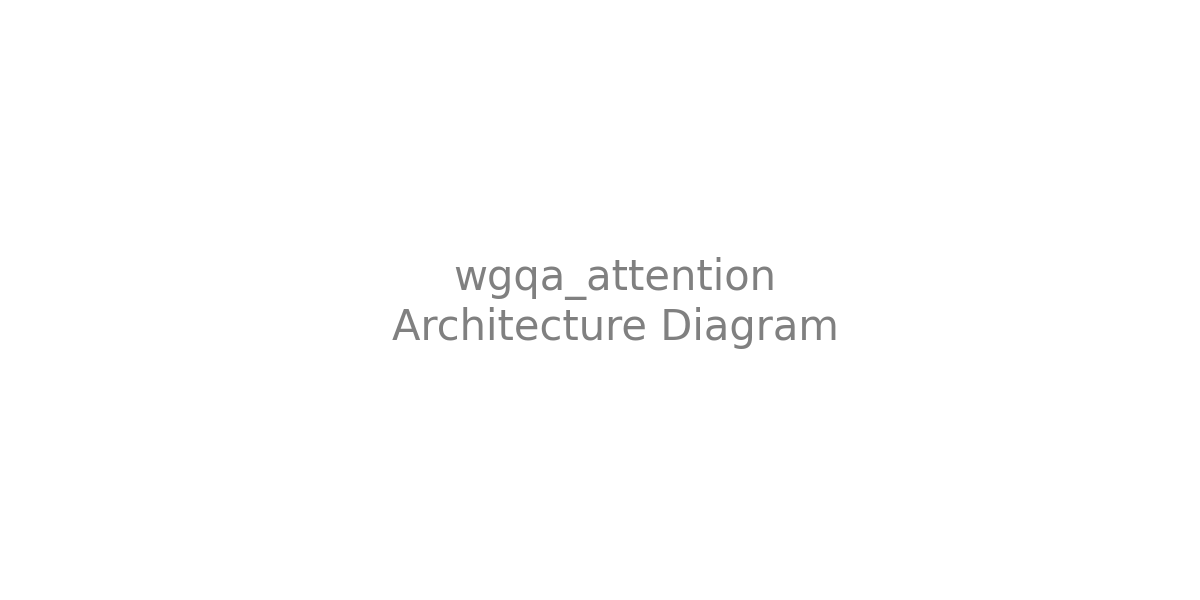
\includegraphics[width=\linewidth]{figures/wgqa_attention_architecture.png}
\caption{Architectural schematic of gqa.}
\label{fig:arch_gqa}
\end{figure}
